% 02/05 changed from .emf to n.png.  Native check
% 02/07 modified typos, eq No, etc. by Makimoto
% 03/12 modified according to 03/07 mail
% 03/22 and 03/25 and 03/26 modified

%%%%%%%%%%%%%%%
%   D-VWAP   %%
%%%%%%%%%%%%%%%

%\setcounter{section}{0}

\chapter{Dynamic Optimal Slice of a VWAP Trade}\label{chap_d}


\begin{quote}
{\bf Abstract} \quad This chapter analyzes an optimal execution strategy of a 
VWAP trade by dynamic control and derives an approximating solution. Non-
negative constraint plays an important role in a dynamic strategy because the 
market trading volume ratio may decrease after big news arrives.  If sell order 
is not allowed, the optimal execution delays in order to avoid excessive execution.  
Also, if the market trading volume surges, the trader should hold his execution 
rather than follow the market trading volume.  We confirm execution error 
reduction by actual trading data.


\end{quote}


%%%%%%%%%%%%%%%%%
\section{Introduction}\label{sec_d1}
VWAP stands for volume-weighted average price during a certain trading period, 
and a VWAP trade refers a trade that uses VWAP as a benchmark.  This chapter 
analyzes the dynamic optimal execution strategy of a VWAP trade.  It extends the 
work of Chapter \ref{chap_s} of this study, which analyzes VWAP trade 
statically.  

As VWAP has become an industry standard, related issues acquire popularity.  
From an empirical side, numerous studies have been done on the relationship 
between price volatility and market trading volume since Clark's (1973) seminal 
paper, including Epps and Epps (1976), Tauchen and Pitts (1983).  Karpoff (1987) 
summarizes these results, and Andersen (1996) proposes a modified model.  These 
studies, in general, support the existence of a positive correlation between 
price volatility and market trading volume and the autocorrelation of themselves 
because surprising news boosts both price volatility and market trading volume.  
Besides, Jain and Joh (1988), Admati and Pfleiderer (1988), Foster and 
Viswanathan (1990), and Chan et al.~(1995) study intraday data and find
a
``U-shaped effect," i.e., within a single day, price volatility and market trading 
volume tend to be higher at the opening and closing than in the middle of a 
trading session. 

Based on these findings, Chapter \ref{chap_s} of this study analyzes optimal 
execution of a VWAP trade.  In executing market trades, a VWAP trader wishes to 
get the average execution price as close to the market VWAP as possible to avoid 
price movement risk.  To do so, a VWAP trader slices a whole trade into small 
executions and tries to spread the executions in a well-balanced manner over the 
trading period, which makes VWAP trades rather labor intensive.  Therefore, it 
often makes sense to build a standard strategy, and execute trades automatically 
according to it.  Although Chapter \ref{chap_s} of this study obtains several 
important implications caused by the correlation between trading volume and 
price volatility, the strategy is optimized statically due to statistical, 
computational, and analytical difficulty.  

However, we might be able to predict the behavior of stocks with frequent trades 
to some extent.  Further, because economic impact tends to be large for such 
stocks, dynamic optimization may reduce considerable execution error further in 
such cases.  Also, it is computationally feasible to apply dynamic control for 
few selected large orders.  Besides, if sell order is not allowed, it is expected that the dynamic optimal execution delays in order to avoid excessive execution.  Therefore, this chapter employs dynamic programming 
and allows traders to change their strategies in the middle of the day after the 
true market trading volume is observed.  

This chapter is organized as follows.  Section \ref{sec_d2} formulizes the 
optimal strategy, and Section \ref{sec_d3} derives the solution.  Finally, 
Section \ref{sec_d4} concludes the analysis.

\section{Formulization of the Optimal Slicing}\label{sec_d2}
Imagine a discrete time frame $t=0,1,\cdots,T$ and a case in which a trader buys 
a certain number of shares and tries to get the average purchase price as close 
as possible to the market VWAP during the trading period from time 1 to time 
$T$.  Let $P_t$ denote the market price at $t\ (t=0,\cdots,T)$, and define
\[
  \Delta P_t \define P_t-P_{t-1}, \qquad t=1,2,\cdots,T.
\]
Let $\Delta v_t$ denote the trader's execution volume at time $t$, and define
\[
  v_t \define \sum_{s=1}^t \Delta v_s, \qquad t=1,2,\cdots,T; \qquad\qquad 
v_0=0.
\]
Also, let $\Delta V_t$ denote the market trading volume at time $t\ 
(t=1,\cdots,T)$ excluding the trader's, and define
\[
  V_t \define \sum_{s=1}^t \Delta V_s, \qquad t=1,2,\cdots,T; \qquad\qquad 
V_0=0,\ \ a.e.
\]
Define the filtration generated by $\{ P_t;\; t=0,1,\cdots,T \}$ and $\{ V_t;\; 
t=0,1,\cdots,T \}$ as
\[
  \calF_t \define \sigma \{ (P_s, V_s); \; s=0,1,\cdots, t \}, \qquad 
t=0,1,\cdots,T.
\]
Under this framework, VWAP trades are executed with the following constraints.

\begin{description}
 \item[(Constraint 1)] At time 0, the trader knows the exogenous whole trade 
size $v_T$, which has to be completed by time $t=T$.
 \item[(Constraint 2)] The trader can submit only buy orders but not sell 
orders, which we call non-negative constraint henceforth.
\[
 0 = v_0 \leq v_1 \leq v_2 \leq \cdots \leq v_{T-1} \leq v_T.
\]
\item[(Constraint 3)] When the trader determines the controllable variable, the 
execution volume $\Delta v_t$ at time $t$, only information up to time $t-1$ is 
available, i.e., $\{ v_t \}$ should be $\{ \calF_t \}$-predictable.
\end{description}
A trader's VWAP is expressed as
\[ %\begin{equation}\label{eq_d1}
  vwap=\frac{\sum_{t=1}^T P_t \Delta v_t}{v_T}.
\] %\end{equation}
Also, the market VWAP excluding the traders' is
\[ %\begin{equation}\label{eq_d2}
  VWAP=\frac{\sum_{t=1}^T P_t \Delta V_t}{V_T}.
\] %\end{equation}
Therefore, the VWAP of the whole market is
\[ %\begin{equation}\label{eq_d3}
  TVWAP=\frac{\sum_{t=1}^T P_t (\Delta V_t + \Delta v_t)}{V_T+v_T}.
\] %\end{equation}
Assume that the trader's execution volume is sufficiently small compared to 
market tradng volume.  Thus, we make the following approximation.

\begin{approximation}\label{appr_d1}
 \quad $V_T/(V_T+v_T) \approx 1,\ \ a.e.$
\end{approximation}

Under this approximation,  
\begin{eqnarray*}
  TVWAP - vwap
   & = & \frac{1}{V_T+v_T} \sum_{t=1}^T P_t \Delta V_t - 
\frac{V_T}{(V_T+v_T)v_T}
         \sum_{t=1}^T P_t \Delta v_t \\
   & \approx & \frac{1}{V_T} \sum_{t=1}^T P_t \Delta V_t - \frac{1}{v_T}
         \sum_{t=1}^T P_t \Delta v_t.
\end{eqnarray*}
Define $y_t \define v_t/v_T\ (t=0,1,\cdots,T)$, and we consider $\{ y_s \}$ as 
the controllable variable rather than $\{ v_s \}$.  The constraints can be 
rewritten as 
\begin{description}
 \item[(Constraint 1')] $y_T=1$.
 \item[(Constraint 2')] $0=y_0 \leq y_1 \leq y_2 \leq \cdots \leq y_{T-1} \leq 
y_T=1$.
 \item[(Constraint 3')] $\{ y_s \}$ is $\{ \calF_s \}$-predictable.
\end{description}
Note that $\displaystyle \{\frac{V_t}{V_T}\}$ is $\calF_T$-measurable but not 
$\{ \calF_t \}$-adapted.
A simple calculation shows that
\begin{eqnarray*}
  \frac{1}{V_T} \sum_{t=1}^T P_t \Delta V_t - \frac{1}{v_T} \sum_{t=1}^T P_t 
\Delta v_t
   & = & \sum_{t=1}^T \left( P_0 + \sum_{s=1}^t \Delta P_s \right)
         \left( \frac{\Delta V_t}{V_T} - \frac{\Delta v_t}{v_T} \right) \\
   & = & \sum_{t=1}^T \sum_{s=1}^t \Delta P_s
         \left( \frac{\Delta V_t}{V_T} - \frac{\Delta v_t}{v_T} \right) \\
   & = & \sum_{s=1}^T \Delta P_s \sum_{t=s}^T
         \left( \frac{\Delta V_t}{V_T} - \frac{\Delta v_t}{v_T} \right) \\
   & = & \sum_{s=1}^T \Delta P_s ( y_{s-1} - \frac{V_{s-1}}{V_T} ) \\
   & = & \sum_{s=1}^{T-1} \Delta P_{s+1} ( y_s - \frac{V_s}{V_T} ).
\end{eqnarray*}
Therefore, 
\begin{eqnarray}
  \ex{(TVWAP-vwap)^2}
   & \approx & \ex{\left( \sum_{s=1}^{T-1} \Delta P_{s+1} (y_s-\frac{V_s}{V_T}) 
\right)^2} \nonumber \\
   & = & \sum_{s=1}^{T-1} \ex{\Delta P_{s+1}^2 (y_s - \frac{V_s}{V_T})^2} 
\nonumber \\ 
   &   & \quad +2 \sum_{s=2}^{T-1} \sum_{t=1}^{s-1}
         \ex{\Delta P_{s+1} \Delta P_{t+1} (y_s-\frac{V_s}{V_T}) (y_t-
\frac{V_t}{V_T})}. \label{eq1_d1}
\end{eqnarray}
Based on empirical analyses such as Jain and Joh (1988), we make the following 
assumptions.

\begin{assumption}\label{ass_d1}

\quad \\
\vspace*{-7mm}

\begin{enumerate}
\item $\Delta P_s=\sigma_{P_s}\epsilon_{P_s}$ where $\epsilon_{P_s}$ is a 
sequence of independent random variables.
\item $\ex{\epsilon_{P_s}}=0, \ex{\epsilon_{P_s}^2}=1 \ (s=1,\cdots,T)$.
\item $\{ \epsilon_{P_s} \}$ is independent of $\{\displaystyle  \frac{V_s}{V_T} 
\}$ and $\{ \sigma_{P_s} \}$.
\end{enumerate}
\end{assumption}
Regarding the first term of (\ref{eq1_d1}), since $y_s$ is
$\calF_{s-1}$-measurabel and independent of $\epsilon_{P_{s+1}}$,
\[ %\begin{equation}
  \ex{\Delta P_{s+1}^2 (y_s-\frac{V_s}{V_T})^2} = \ex{\sigma_{P_{s+1}}^2 (y_s-
\frac{V_s}{V_T})^2}.
\] %\end{equation}
Regarding the second term of (\ref{eq1_d1}), for $s>t$,
\[ %\begin{equation}
  \ex{\Delta P_{s+1} \Delta P_{t+1} (y_s-\frac{V_s}{V_T}) (y_t-\frac{V_t}{V_T})}
   = \ex{\epsilon_{P_{s+1}}} \ex{\epsilon_{P_{t+1}} \sigma_{P_{s+1}} 
\sigma_{P_{t+1}} (y_s-\frac{V_s}{V_T}) (y_t-\frac{V_t}{V_T})} = 0.
\] %\end{equation}
Therefore, the objective function to minimize is given by
\begin{equation}\label{eq1_d2}
  \ex{(TVWAP-vwap)^2} \approx \sum_{s=1}^{T-1} \ex{\sigma_{P_{s+1}}^2 (y_s-
\frac{V_s}{V_T})^2}.
\end{equation}
Note that without the non-decreasing constraint for $\{ y_s \}$, $\displaystyle 
y_s = \cex{\frac{V_s}{V_T}}{\calF_{s-1}}$ is the optimal execution strategy.  
However, in a dynamic strategy, the non-decreasing constraint plays an important 
role in increasing the risk of the excessive execution risk because $\displaystyle \frac{V_s}{V_T}$ may decrease after big news arrives 
and the market trading volume surges while $\displaystyle \ex{\frac{V_s}{V_T}}$ 
is generally monotone increasing in a static strategy.

We decompose the sequence $\displaystyle \{ \frac{V_s}{V_T} \}$, which is not 
observed accurately, into a observable part and an error part as
\[ %\begin{equation}
  \frac{V_s}{V_T} = Y_s + \epsilon_{V_s}, \qquad Y_s \define 
\cex{\frac{V_s}{V_T}}{\calF_s},
  \qquad s=1,2,\cdots,T-1; \qquad\qquad \epsilon_{V_T} = 0, \ \ a.e,
\] %\end{equation}
where we make some regular asumptions for the error part.

\begin{assumption}\label{ass_d2}
\quad \\
\vspace*{-7mm}
\begin{enumerate}
\item $\{ \epsilon_{V_s} \}$ is a sequence of independent random variables.
\item $\ex{\epsilon_{V_s}} = 0\ (s=1,\cdots,T-1)$.
\item $\{ \epsilon_{V_s} \}$ and $\{ Y_s \}$are independent.
\end{enumerate}
\end{assumption}
Since $\{ y_s \}$ is $\{ \calF_{s} \}$-predictable, $\{ y_s \}$ is
independent of $\{ \epsilon_{V_s} \}$.  Therefore, 
\begin{eqnarray}
  \ex{\sigma_{P_{s+1}}^2 (y_s-\frac{V_s}{V_T})^2}
  & = & \ex{\sigma_{P_{s+1}}^2 \{(y_s-Y_s) - \epsilon_{V_s}\}^2} \nonumber \\
  & = & \ex{\sigma_{P_{s+1}}^2 (y_s-Y_s)^2} - 2 \ex{\sigma_{P_{s+1}}^2 (y_s-
Y_s)}\ex{\epsilon_{V_s}} + \ex{\sigma_{P_{s+1}}^2\epsilon_{V_s}^2} \nonumber \\
  & = & \ex{\sigma_{P_{s+1}}^2 (y_s-Y_s)^2} + 
\ex{\sigma_{P_{s+1}}^2\epsilon_{V_s}^2}. \label{eq1_d3}
\end{eqnarray}
Since the second term of (\ref{eq1_d3}), $\ex{\sigma_{P_{s+1}}^2 
\epsilon_{V_s}^2}$, is not controllable, the objective function to minimize in 
(\ref{eq1_d2}) is given by
\[ %\begin{equation}
  \sum_{s=1}^{T-1}  \ex{\sigma_{P_{s+1}}^2 (y_s - Y_s)^2}.
\] %\end{equation}




%%%%%%%%%%%%%%%%%%
\section{Derivation of the Optimal Strategy}\label{sec_d3}

\subsection{Uncorrelated Case}
In order to formulize our optimization problem as a linear Markov decision 
process, we make the following assumption.

\begin{assumption}\label{ass_d3}
 \quad $\{ Y_s \}$ is a Markov chain.
\end{assumption}

The state is represented as the pair of the trader's execution ratio and the 
observed market trading volume ratio $(y_s,Y_s)$.  If we write the state at time 
$s$ as $(y_s,Y_s)=(u,w)$, the execution proceeds as follows:

\begin{enumerate}
 \item According to the value of $Y_s$, $y_{s+1}$ is determined, satisfying $y_s 
\leq y_{s+1} \leq 1$.
 \item Under $Y_s=w$, $Y_{s+1}$ is given by the Markov chain.  Also, $P_{s+1}$ 
is given.
 \item $y_{s+1}$ and $Y_{s+1}$ are executed at price $P_{s+1}$, and the state 
moves to $(y_{s+1}, Y_{s+1})$.
\end{enumerate}
If we define
\[ %\begin{equation}
  C_t^*(u,w) \define \min_{u \leq y_t \leq \cdots \leq y_{T-1} \leq 1} \ \ 
    \sum_{s=t}^{T-1} \cex{\sigma_{P_{s+1}}^2 (y_s - Y_s)^2}{Y_{t-1}=w}, \qquad
    t=1,\cdots,T-1
\] %\end{equation}
where the superscript $*$ denotes the optimal solution henceforth.  Bellman 
equation is given by 
\begin{eqnarray}
  \lefteqn{C_t^*(u,w) = \min_{u \leq y_t \leq 1} \ \ \left\{
     \cex{\sigma_{P_{t+1}}^2 (y_t-Y_t)^2}{Y_{t-1}=w} + 
\cex{C_{t+1}^*(y_t,Y_t)}{Y_{t-1}=w} \right\},} \label{eq_d11} \\
  & & \hspace*{10cm} t=1,2,\cdots,T-2. \nonumber
\end{eqnarray}
Since this formula is still too complicated to generate implications, further 
assumptions are made which are considered reasonable based on standard theories 
and empirical analyses.  Firstly, since $Y_0=0$, $Y_T=1$, and $Y_t$ moves 
randomly between time 0 to $T$, we assume $\{ Y_t \}$ is a Brownian bridge.  Secondly, when we fix $w$, $C_{T-1}^*(u,w)$ is a quadratic function of $u$ over the minimum, or a constant otherwise,  it is natural to approximate $C_t$ quadratically.  
Therefore, we made the following assumptions.
\begin{assumption}\label{ass_d4}
\quad \\
\vspace*{-7mm}
\begin{enumerate}
\item The process of $Y_t$ is represented as
\[ %\begin{equation}\label{eq_d8}
Y_t= \bar \eta_t(Y_{t-1})+\sigma_{Y_t}\epsilon_{Y_t}; \qquad Y_0=0, \quad Y_t=1
\] %\end{equation}
where $\bar \eta_t(\, \cdot\, )$ is a linear function, and $\{ \epsilon_{Y_t} \}$ is 
a sequence of normal random variables that is uncorrelated with 
$\{\epsilon_{P_t}\}$.
\item The market trading volume can be predicted precisely enough that 
$\sigma_{Y_t}$ is sufficiently small.
\item  The value function in the Bellman equation can be written as 
\[ %\begin{equation}\label{eq_d11}
  C_{t+1}^*(u, w) = \left\{
  \begin{array}{ll}
   g_t(w), \\
   (a_t w + b_t u + c_t)^2 + g_t(w), 
  \end{array}
  \right. \quad
  \begin{array}{ll}
    w \geq -\frac{b_tu+c_t}{a_t},\\
    w < -\frac{b_tu+c_t}{a_t}
  \end{array}
\] %\end{equation}
for some coefficients $\{ a_t \}$, $\{ b_t \}$, $\{ c_t \}$, and a function $\{ g_t(w) \}$, which is independent of $u$.
\end{enumerate}
\end{assumption}
Further, let $\{\sigma_{P_t}\}$ be uncorrelated with $\{\epsilon_{Y_t}\}$ in 
this subsection while the correlated case is analyzed in Subsection 
\ref{sec_d32}.  
 In this case, (\ref{eq_d11}) is reduced to
\begin{eqnarray*} %\label{eq_d12}
  C_t^* (u, w)
  & = & \min_{u \leq y_t \leq 1} \left\{
        \ex{\sigma_{P_{t+1}}^2} \cex{(y_t-Y_t)^2}{Y_{t-1}=w}
        + \int_{-\infty}^\infty g_t (\eta) f_t(\eta - \bar \eta_t(w)) d \eta
        \right. \\
  &   & \hspace*{5.5cm} \left.
        + \int_{-\infty}^{-(b_t y_t + c_t)/a_t} (a_t \eta + b_t y_t + c_t )^2
        f_t(\eta - \bar \eta_t(w)) d \eta
        \right\} \\
  & = & \min_{u \leq y_t \leq 1} \left\{ \ex{\sigma_{P_{t+1}}^2} (y_t-\ex{Y_t})^2 + I_t + const \right\}
\end{eqnarray*}
where $\displaystyle f_t(x) \define \frac{1}{\sqrt{2\pi}\sigma_{Y_t}}\mboxexp(-\frac{x^2}{2\sigma_{Y_t}^2})$,
\[
 I_t \define \int_{-\infty}^{-(b_t y_t + c_t)/a_t} (a_t \eta + b_t y_t + c_t )^2
        f_t(\eta - \bar \eta_t(w)) d \eta
\]
and
\[
 const \define \int_{-\infty}^\infty g_t (\eta) f_t(\eta - \bar \eta_t(w)) d \eta
\]
which is constant in $y_t$.
Define $\zeta \equiv \eta-\bar \eta_t(Y_{t-1})$, $z_t \equiv -(b_ty_t+c_t)/a_t-
\bar\eta_t(Y_{t-1})$ and $\displaystyle F_t(x)= \int_{-\infty}^x f_t(y) dy$.
Then,
\[ %\begin{equation}\label{eq_d13}
  I_t = \int_{-\infty}^{z_t}a_t^2(\zeta-z_t)^2f_t(\zeta)d\zeta = a_t^2 \int_{-
\infty}^{z_t} (\zeta^2-2z_t\zeta+z_t^2)f_t(\zeta)d\zeta.
\] %\end{equation}
Using the following equations,
\begin{eqnarray*}
  \int_{-\infty}^{z_t} \zeta f_t(\zeta)d\zeta & = & -\sigma_{Y_t}^2 
f_t(z_t),\label{eq_d14}\\
  \int_{-\infty}^{z_t} \zeta^2 f_t(\zeta)d\zeta & = & \sigma_{Y_t}^2 F_t(z_t)-
\sigma_{Y_t}^2 z_t f_t(z_t),\label{eq_d15}
\end{eqnarray*}
we obtain
\[
  I_t =  a_t^2 \sigma_{Y_t}^2 \{(1+z_t^2)F_t(z_t)+z_t f_t(z_t)\}.
\]
Since $\sigma_{Y_t}$ is small, the risk of the excessive execution is expected to be low, which makes $z_t$ small.  Consequently, $I_t$ can be approximated as
\begin{eqnarray*}
  I_t & \simeq & I_t(0)+I_t'(0)z_t+\frac{I_t''(0)}{2}z_t^2 \\
      & \simeq & \frac{a_t^2 \sigma_{Y_t}^2}{2}+\sqrt{\frac{2}{\pi}}a_t^2 
\sigma_{Y_t}z_t+\frac{a_t^2 \sigma_{Y_t}^2}{2}z_t^2.
\end{eqnarray*}
Therefore, the quadratic approximation of $C_t^*(u,w)$ is given by 
\begin{eqnarray*} %\begin{equation}\label{eq_d21}
 C_t^*(u,w)
  & = & \min_{u \leq y_t \leq 1} \left[
        \left\{ \frac{b_t^2 \sigma_{Y_t}^2}{2}+\ex{\sigma_{P_{t+1}}^2} \right\} y_t^2 \right. \\
  &   & \hspace*{1.5cm}
        \left. +\left\{\left(a_tb_t\sigma_{Y_t}^2-2\ex{\sigma_{P_{t+1}}^2}\right)\bar \eta(w) 
        +b_tc_t\sigma_{Y_t}^2-\sqrt{\frac{2}{\pi}}a_tb_t\sigma_{Y_t}\right\}y_t+const \right] \\
  & = & \left\{
  \begin{array}{ll}
   g_{t-1}(w), \qquad w \geq -\frac{b_{t-1}u+c_{t-1}}{a_{t-1}},\\
   (a_{t-1}w+b_{t-1}u+c_{t-1})^2+g_{t-1}(w),
   \qquad w < -\frac{b_{t-1}u+c_{t-1}}{a_{t-1}}
  \end{array}
  \right.
\end{eqnarray*} %\end{equation}
where the minimum is attained by
\[
  y_t= \max\left\{-\frac{\left(a_tb_t\sigma_{Y_t}^2-2\ex{\sigma_{P_{t+1}}^2}\right)
   \bar \eta(w)+b_tc_t\sigma_{Y_t}^2-\sqrt{\frac{2}{\pi}}a_tb_t\sigma_{Y_t}}{b_t^2 
   \sigma_{Y_t}^2+2\ex{\sigma_{P_{t+1}}^2}}, \ u \right\}.
\] %\end{equation}
Therefore, the optimal $\{ y_t^* \}$ is solved iteratively starting with $y_0^* = 0$.

Specifically, if $\bar \eta(u)=\alpha_t+\beta_t u$, then
\[ %\begin{equation}\label{eq_d24}
  y_t^*= \max(d_tY_{t-1}+e_t, y_{t-1}^*), \qquad t = 1,2,\cdots,T-1
\] %\end{equation}
where 
\begin{eqnarray*}
  y_0^* & = & 0,\\
  d_t & = & -\frac{\left(a_tb_t\sigma_{Y_t}^2-
2\ex{\sigma_{P_{t+1}}^2}\right)}{b_t^2 
\sigma_{Y_t}^2+2\ex{\sigma_{P_{t+1}}^2}}\beta_t,\\
  e_t & = & -\frac{\left(a_tb_t\sigma_{Y_t}^2-
2\ex{\sigma_{P_{t+1}}^2}\right)\alpha_t+b_tc_t\sigma_{Y_t}^2-
\sqrt{\frac{2}{\pi}}a_tb_t\sigma_{Y_t}}{b_t^2 
\sigma_{Y_t}^2+2\ex{\sigma_{P_{t+1}}^2}},\\
  a_T & = & b_T \ \ = \ \ c_T \ \ = \ \ 0,\\
  a_{t-1} & = & \frac{a_tb_t\sigma_{Y_t}^2-2\ex{\sigma_{P_{t+1}}^2}}{2b_{t-
1}}\beta_t,\\
  b_{t-1} & = & \sqrt{\frac{b_t^2 \sigma_{Y_t}^2}{2}+\ex{\sigma_{P_{t+1}}^2}},\\
  c_{t-1} & = & \frac{b_tc_t\sigma_{Y_t}^2}{2b_{t-1}}.
\end{eqnarray*}
For example, if $\{ Y_t \}$ is a Brownian bridge, 
\[ %\begin{equation}\label{eq_d25}
dY_t=dB_t+\frac{1-Y_t}{1-t}dt
\] %\end{equation}
and therefore,
\[ %\begin{equation}\label{eq_d26}
\bar \eta(Y_{t-1})-Y_{t-1}=\frac{1-\bar \eta(Y_{t-1})}{1-t} \Delta t
\] %\end{equation}
or, equivalently,
\[ %\begin{equation}\label{eq_d27}
\bar \eta(Y_{t-1})=\frac{1-t}{1-t+\Delta t}Y_{t-1}+\frac{\Delta t}{1-t+\Delta 
t}. 
\] %\end{equation}
Substituting into the general solution, we obtain
\[ %\begin{equation}\label{eq_d28}
 y_t^* = \max(d_tY_{t-1}+e_t,y_{t-1}^*), \qquad t = 1,2,\cdots,T-1
\] %\end{equation}
where 
\begin{eqnarray*}
  y_0^* & = & 0,\\
  d_t & = & -\frac{\left(a_tb_t\sigma_{Y_t}^2-
2\ex{\sigma_{P_{t+1}}^2}\right)}{b_t^2 
\sigma_{Y_t}^2+2\ex{\sigma_{P_{t+1}}^2}}\frac{1-t}{1-t+\Delta t},\\
  e_t & = & -\frac{\left(a_tb_t\sigma_{Y_t}^2-2\ex{\sigma_{P_{t+1}}^2}\right)\frac{\Delta t}{1-t+\Delta 
t}+b_tc_t\sigma_{Y_t}^2-\sqrt{\frac{2}{\pi}}a_tb_t\sigma_{Y_t}}{b_t^2 
\sigma_{Y_t}^2+2\ex{\sigma_{P_{t+1}}^2}}.
\end{eqnarray*}
As we have mentioned, the non-decreasing constraint plays an important role in a 
dynamic strategy because $Y_t$ may decrease after some big news arrives and the 
market trading volume surges while $\ex{Y_t}$ is generally monotone increasing 
in a static strategy.

In order to avoid excessive execution, $y_t^*$ is expected to be smaller than $Y_t$, 
the optimal strategy without non-decreasing constraint.  Also, once news arrives, 
and $Y_t$ happens to decrease, $y_t^*$ stays constant until $Y_t$ gets back 
large enough.  Therefore, if the market trading volume surges, the trader should 
hold his execution rather than follow the market trading volume.

Figure \ref{fg_d1} shows $Y_t$ and $y_t^*$, and Figure \ref{fg_d2} shows $g_t$ 
and $h_t$ for $\sigma_{Y_t}=1$ and all the $\epsilon_{Y_t}$ are zero.  We can 
see that $y_t^*$ is smaller than $Y_t$ due to the risk that $Y_t$ decreases, 
which delays trade execution.  This is more significant for larger 
$\sigma_{Y_t}$.

\begin{figure}[htbp]
\begin{center}
 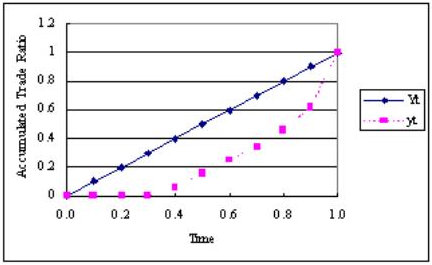
\includegraphics[width=10cm,height=6cm]{fg_d1n.png}
\end{center}
\caption[Numerical example of $Y_t$ and $y_t^*$]{{\bf Numerical example of $Y_t$ 
and $y_t^*$ for $\sigma_{Y_t}=1$ and
where all the $\epsilon_{Y_t}$ are zero.}
 \quad We can see that $y_t^*$ is smaller than $Y_t$ due to the risk that $Y_t$ 
decreases, which delays trade
execution.
 This is more significant for larger $\sigma_{Y_t}$.}\label{fg_d1}
\end{figure}

\begin{figure}[htbp]
\begin{center}
  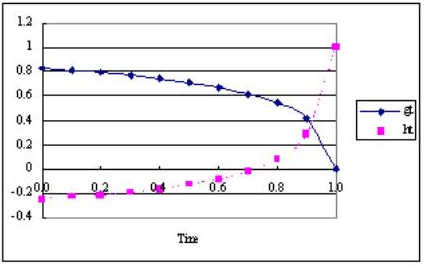
\includegraphics[width=10cm,height=6cm]{fg_d2n.png}
\end{center}
\caption[$g_t$ and $h_t$ for $\sigma_{Y_t}=1$.]{{\bf $g_t$ and $h_t$ for 
$\sigma_{Y_t}=1$.}
 \quad $g_t$ and $h_t$ are deterministic functions that depends only on 
$\sigma_{Y_t}=1$.}\label{fg_d2}
\end{figure}


\subsection{Correlated Case}\label{sec_d32}
If we take correlation between $Y_t$ and $\sigma_{P_t}$ into account, the 
following equation holds.
\begin{eqnarray*}\label{eq_d29}
  \sum_{t=0}^T \ex{(Y_t-y_t)^2 \sigma_{P_{t+1}}^2}
  & = & \sum_{t=0}^T 
\ex{\left\{\frac{\ex{Y_t\sigma_{P_{t+1}}^2}}{\ex{\sigma_{P_{t+1}}^2}}-
y_t\right\}^2 }\ex{\sigma_{P_{t+1}}^2} \nonumber \\
  & = & \sum_{t=0}^T 
\ex{\left\{\ex{Y_t}+\frac{\mbox{Cor}(Y_t,\sigma_{P_{t+1}}^2)\sigma_{Y_t} 
\mbox{Std}(\sigma_{P_{t+1}}^2)}{\ex{\sigma_{P_{t+1}}^2}}-y_t\right\}^2 } 
\ex{\sigma_{P_{t+1}}^2}
\end{eqnarray*}
where $\mbox{Cor}$ and $\mbox{Std}$ stands for the correlation and the standard 
deviation, respectively.  Let the superscript $**$ denote the optimal solution 
of the correlated case.  Then, if $\mbox{Cor}(Y_t,\sigma_{P_{t+1}}^2)$ and 
$\mbox{Std}(\sigma_{P_{t+1}}^2)$ are deterministic, we can solve $y_t^{**}$ just 
as previous argument as
\[ %\begin{equation}\label{eq_d30}
y_t^{**}=y_t^*+\frac{\mbox{Cor}(Y_t,\sigma_{P_{t+1}}^2)\sigma_{Y_t}\mbox{Std}
(\sigma_{P_{t+1}}^2)}{\ex{\sigma_{P_{t+1}}^2}}.
\] %end{equation}

\subsection{Back Tests}
Next, we confirm our theoretical results empirically, using actual intraday data 
from the Tokyo Stock Exchange provided by Nikkei Quick Information Co.~Ltd.  All 
empirical analyses in this chapter are based on trading data from October 2000 
to March 2001 on the 10 stocks with the largest market capitalization.  Data 
from December 29, 2000 and January 4, 2001 are excluded since there was no 
afternoon session on these days.  We chose these large stocks in order to retain 
statistical accuracy since their ticks are frequent and stable.  We believe that 
results can be applied to other stocks since the relationship between price 
volatility and market trading volume is ubiquitous for all stocks as Chan et al. 
(1995) pointed out.  We assume that accumulated market trading volume follows 
the linear difference equation as 
\[ %\begin{equation}\label{eq_d31}
  \bar \eta(u)=\alpha_t+\beta_t u
\] %\end{equation}
and the coefficients $\alpha$ and $\beta$ are obtained through ordinary least 
square regressions where realized $\displaystyle \frac{V_t}{V_T}$ is used as the 
estimate of $Y_t$.  Executions are allocated to periods according to each 
strategy, and the trade is assumed to be executed at the VWAP of the 
corresponding period.  Static strategy is performed in the exactly same manner 
as in Chapter \ref{chap_s}.

Table \ref{table_d1} shows VWAP execution errors for each stock.  We can see 
that dynamic optimization effectively reduces VWAP execution errors.  Also, we 
can further improve our results by taking correlation between accumulated market 
trading volume ratio and price volatility.  In practice, we suffer further price 
changes within the interval and discritization errors due to the minimum trading 
unit, both of which are considered to be proportional to the price volatility as 
in the static optimization in Chapter \ref{chap_s}.

Also, Figure \ref{fg_d3} shows the average delay of the optimal executions, 
$Y_t- y_t^*$ for the uncorrelated case and $Y_t- y_t^{**}$ for the correlated 
case.  We can see that the risk of $Y_t$ decrease and the correlation between 
price volatility and trading volume indeed delays the optimal trade execution.


\begin{table}[htbp]
\begin{center}
\begin{tabular}{|l||c|c|c|} \hline
 & Static & Dynamic & Dynamic (Correlated) \\ \hline\hline
 Takeda & 0.00102 & 0.00071 & 0.00071 \\ \hline
 Matsushita & 0.00095 & 0.00039 & 0.00039 \\ \hline
 Sony & 0.00093 & 0.00044 & 0.00044 \\ \hline
 Toyota & 0.00100 & 0.00059 & 0.00058 \\ \hline
 Honda & 0.00121 & 0.00083 & 0.00083 \\ \hline
 Seven-Eleven Japan & 0.00219 & 0.00167 & 0.00167 \\ \hline
 Mizuho	& 0.00143 & 0.00092 & 0.00092 \\ \hline
 Tokyo-Mitsubishi & 0.00133 & 0.00077 & 0.00076 \\ \hline
 Nomura & 0.00142 & 0.00065 & 0.00064 \\ \hline
 NTT & 0.00176 & 0.00058 & 0.00059 \\ \hline
 NTT Docomo & 0.00128 & 0.00050 & 0.00050 \\ \hline
 Tokyo Electric Power & 0.00065 & 0.00042 & 0.00041 \\ \hline\hline
 Average & 0.00127 & 0.00071 & 0.00070 \\ \hline
\end{tabular}
\end{center}
\caption[Delay of the optimal execution]{{\bf Delay of the optimal execution.}
 \quad This graph shows the delay of the optimal execution from the average 
trading volume ($y$-axis), which coincides with $Y_t- y_t^*$ in the Uncorrelated 
Case and $Y_t- y_t^{**}$ in the Correlated Case in each period ($x$-axis).  We 
can see that the risk of $Y_t$ decrease and the correlation between price 
volatility and trading volume indeed delays the optimal trade 
execution.}\label{table_d1}
\end{table}


\begin{figure}[htbp]
\begin{center}
 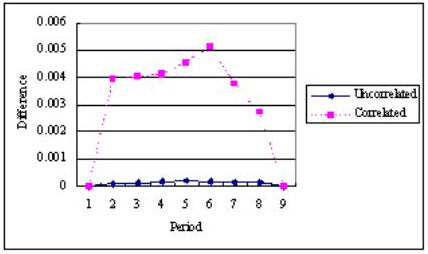
\includegraphics[width=10cm,height=6cm]{fg_d3n.png}
\end{center}
\caption[Graph of VWAP execution errors]{{\bf This graph shows VWAP execution 
errors for each stock.}
 \quad We can see that dynamic optimization effectively reduces VWAP execution 
errors.
 Also, we can further improve our results by taking correlation between 
accumulated market trading volume ratio
 and price volatility.}\label{fg_d3}
\end{figure}


%%%%%%%%%%%%%%%%%%%%
\section{Closing Remarks}\label{sec_d4}
In this chapter we analyzes an optimal execution strategy of a VWAP trade by 
dynamic control and derives approximating solution. Non-negative constraint 
plays an important role in a dynamic strategy because the market trading volume 
ratio may decrease after big news arrives.  If sell order is not allowed, the 
optimal execution delays in order to avoid excessive execution.  Also, if the market 
trading volume surges, the trader should hold his execution rather than follow 
the market trading volume.  We confirm execution error reduction by actual 
trading data.

For simplicity, this analysis studies only one asset execution but not multiple 
asset execution with diversification effect.  Also, estimating the market 
trading volume may not be an easy task even with qualitative judgment.  These 
issues are left for further analysis.
